\documentclass[a4paper,10pt]{corsage}

\title{\Huge{}El protocolo IPv6\\\large{}Administración de Redes Locales\footnote{Imágenes disponibles en \texttt{https://github.com/zkolsh/rloc-ipv6/tree/main/graphics}}}
\author{Mateo Delmagro}
\date{Mar 2025}

\usepackage{amsmath}
\usepackage{amssymb}
\usepackage[spanish]{babel}
\usepackage{bytefield}
\usepackage{graphicx}
\usepackage[utf8]{inputenc}
\usepackage[loversize=0.25]{lettrine}
\usepackage{needspace}
\usepackage[defaultlines=3, all]{nowidow}
\usepackage{tcolorbox}
\usepackage{xcolor}

\definecolor{information-line}{HTML}{FF4040}
\definecolor{information-background}{HTML}{FFE0E0}

\graphicspath{{./graphics/}}

\bytefieldsetup{bitwidth=3mm} \bytefieldsetup{boxformatting={\centering\ttfamily}}

\newcommand{\ipaddress}[1]{\texttt{#1}}
\newcommand{\macaddress}[1]{\ipaddress{#1}}
\newcommand{\devname}[1]{\textsc{#1}}

\makeatletter
\newcommand*{\@doendeq}{%
	\everypar{{\setbox\z@\lastbox}\everypar{}}%
}
\makeatother

\newcommand{\rest}{%
	\par\vspace{0.5\baselineskip}%
	\centerline{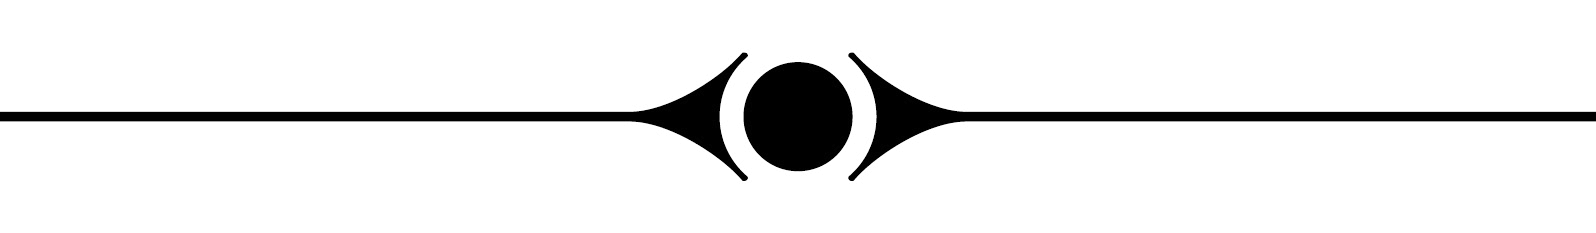
\includegraphics[height=\baselineskip]{rest}}%
	\vspace{\parskip}\vspace*{-\parskip}%
	\ignorespacesafterend\par\noindent\aftergroup%
}

\newcommand{\pant}{%
	\par\vspace*{-\parskip}\vspace{0.8\baselineskip}%
	\centerline{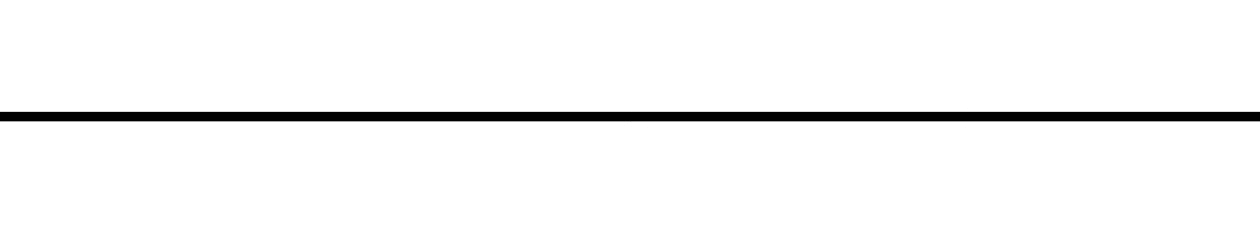
\includegraphics[height=\baselineskip]{pant}}%
	\vspace*{-\parskip}\vspace{0.8\parskip}%
	\ignorespacesafterend\par\noindent\aftergroup
}

\makeatletter
\newenvironment{information}{%
	\begin{tcolorbox}[
		left skip=50mm,
		right skip=50mm,
		left=8pt,
		right=8pt,
		top=3\parskip,
		bottom=2\parskip,
		colback=information-background,
		colframe=information-line,
		boxrule=0pt,
		leftrule=4pt,
		sharp corners=all
	]%
}{%
	\end{tcolorbox}%
	\ignorespacesafterend\par\noindent\aftergroup\@doendeq%
}

\newenvironment{console}{%
	\begin{tcolorbox}[
		left skip=1cm,
		right skip=1Cm,
		left=8pt,
		right=8pt,
		top=2.5\parskip,
		bottom=2\parskip,
		colback=gray!10,
		colframe=gray!40,
		boxrule=0pt,
		leftrule=4pt,
		sharp corners=all,
		fontupper=\ttfamily\flushleft\footnotesize
	]%
}{%
	\end{tcolorbox}%
	\ignorespacesafterend\par\noindent\aftergroup\@doendeq%
}

\makeatother

\begin{document}
\pagenumbering{roman}
\maketitle
\cleardoublepage

\pagenumbering{arabic}
\newcommand{\scenarioheight}{5\baselineskip}
\chapter{Autoconfiguración de dispositivos}
	\lettrine{E}{n este trabajo}, vamos a estudiar el comportamiento del protocolo IPv6.  El mismo es la versión más reciente del protocolo IP, diseñado para solucionar el problema del agotamiento de direcciones IPv4.  Buscó solucionar esto abandonando algunas ideas de la versión anterior---como la notación punteada, las direcciones de broadcast, etc---e incorporando otras ideas nuevas, como por ejemplo la \textit{stateless address autoconfiguration} (SLAAC) para la autoconfiguración de los dispositivos, la cual nos gustaría ver ahora.

	Para ello, comencemos con el siguiente escenario:
	\begin{figure}[h]
		\centering
		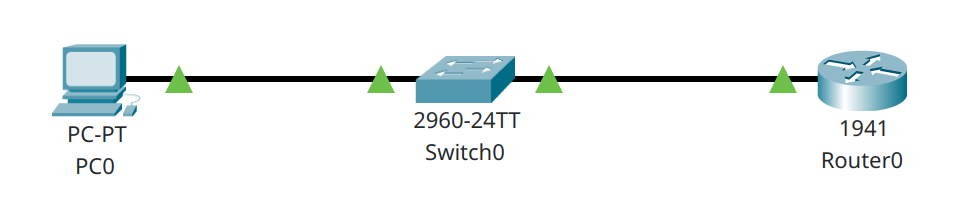
\includegraphics[height=\scenarioheight]{slaac-quiet}
	\end{figure}

	Aquí tenemos una computadora conectada a un router mediante un switch.  Para ver como SLAAC hace que la \devname{PC0} se autoconfigure, debemos primero activar el ruteo IPv6 en la red---entonces entramos a la configuración del router:
	\begin{console}
		\verb|Router(config)# ipv6 unicast-routing|
	\end{console}

	Y ahora debemos configurar sus direcciones.  En IPv6 una misma placa puede tener varias direcciones---por ejemplo, va a tener una \textit{dirección de enlace local} (LLA) no ruteable, la cual veremos que tiene un cierto parecido con las direcciones de la Capa 2.  Además, queremos que el router tenga una dirección GUA (\textit{Global Unique Address}), que son como una IPv4 pública:
	\begin{console}
		\begin{verbatim}Router(config)# interface g0/0
Router(config-if)# ipv6 enable
Router(config-if)# ipv6 address fe80::1 link-local
Router(config-if)# ipv6 address 2001:db8:acad:1::1/64
Router(config-if)# no shutdown\end{verbatim}
	\end{console}

	Hecho esto, \devname{Router0} podrá enviar y recibir mensajes IPv6---Y, como lo indica el protocolo, comenzará a participar en mecanismos que le permiten a los hosts realizar SLAAC.

	\pant

	En términos generales, la autoconfiguración mediante SLAAC se ordena en cuatro pasos principales.  Primero, el host envía un mensaje de \textit{Router Solicitation}.  En respuesta a ese mensaje---o a veces periódicamente por su cuenta---el router responderá con un mensaje de \textit{Router Advertisement}.  Con esta información, el host autoconfigura sus direcciones de enlace local y global de forma tentativa, y luego envía un mensaje de \textit{Neighbor Solcitation} para asegurarse que ningún otro host en la red haya elegido esa dirección.  Si las direcciones están libres, entonces las adquiere como suyas.

	Como dije, \devname{Router0} ya está participando de SLAAC, asi que podemos ver los mensajes \textit{Router Advertisement} (RA) que está enviando periódicamente si le decimos que los imprima en la consola.  Se pueden ver los contenidos de este mensaje de forma visual en más detalle en la Figura \ref{fig:icmp-ra}, la cual se sugiere consultar ahora.
	\begin{console}
		\verb|Router# debug ipv6 nd|

		\verb|ICMP Neighbor Discovery events is on|
	\end{console}

	\begin{console}
		\begin{verbatim}ICMPv6-ND: (GigabitEthernet0/0, FE80::1) send RA to FF02::1
ICMPv6-ND: (GigabitEthernet0/0, FE80::1) Sending RA(1800) to FF02::1
ICMPv6-ND:     MTU = 1500
ICMPv6-ND:     prefix = 2001:DB8:ACAD:1::/64 [LA] 2592000/604800\end{verbatim}
	\end{console}

	\begin{figure}
		\centering
		\begin{bytefield}{32}
			\bitbox{4}{Ver: 6} & \bitbox{8}{TRFC} & \bitbox{20}{Flow label} \\
			\bitbox{16}{Payload length: 60 bytes} & \bitbox{8}{Next: 0x3a} & \bitbox{8}{Hop lim. 255} \\
			\wordbox{4}{Source IP:  \ipaddress{fe80::1}} \\
			\wordbox{4}{Destination IP:  \ipaddress{ff02::1}} \\

			\\

			\bitbox{8}{Type: 134} & \bitbox{8}{Code: 0} & \bitbox{16}{Checksum: 0} \\
			\bitbox{8}{Hop lim.: 64} & \bitbox{1}{\tt M} & \bitbox{1}{\tt O} & \bitbox{6}[bgcolor=lightgray]{} & \bitbox{16}{Router lifetime: 1800s.} \\
			\wordbox{1}{Reachable time: 0 (inespecificado)} \\
			\wordbox{1}{Retransmission timer: 0 (inespecificado)} \\

			\\

			\bitbox{8}{Type: 1\\\scriptsize{Link layer}} & \bitbox{8}{Length: 1} & \bitbox[lrt]{16}{} \\
			\wordbox[lrb]{1}{MAC Address: \macaddress{00:0b:be:46:4a:01}} \\

			\\

			\bitbox{8}{Type: 5\\\scriptsize{MTU}} & \bitbox{8}{Length: 1} & \bitbox{16}[bgcolor=lightgray]{} \\
			\wordbox{1}{Maximum Transmission Unit: 1500} \\

			\\

			\bitbox{8}{Type: 3\\\scriptsize{Pfx. info.}} & \bitbox{8}{Length: 4} & \bitbox{8}{Pfx. len.: 1} & \bitbox{1}{L} & \bitbox{1}{A} & \bitbox{6}[bgcolor=lightgray]{} \\
			\wordbox{1}{Valid lifetime:  2592000 segundos (30 días)} \\
			\wordbox{1}{Preferred lifetime:  604800 segundos (7 días)} \\
			\wordbox{1}[bgcolor=lightgray]{} \\
			\wordbox{4}{Prefix: \ipaddress{2001:db8:acad:1::64}}
		\end{bytefield}
		\caption{Router Advertisement de \devname{Router0}.}
		\label{fig:icmp-ra}
	\end{figure}

	Tratemos de darle sentido a todo esto.  Primero, vemos uqe la dirección IP de salida es \ipaddress{fe80::1}---la misma que habíamos establecido como enlace local en esa interface.  Esto le sirve al host para aprender dónde está el gateway, y opcionalmente en este mensaje el router puede incluír su dirección MAC para que los hosts no tengan que buscarla de nuevo.  ¿Qué podríamos poner para la dirección de destino?  La idea de este mensaje es que sea enviado a todos los dispositivos en la red---en IPv4 llamaríamos a esto un broadcast, pero como habíamos mencionado, estas direcciones desaparecieron en IPv6.  En su lugar, usamos la dirección \ipaddress{ff02::1}, o \textit{all nodes multicast}, que es enviada a todos los dispositivos IPv6 y no es enviado fuera del enlace local.

	El tipo del mensaje ICMP es \texttt{134} (RA), y dentro de su contenido se podrán encontrar los prefijos IPv6 de cada red---en nuestro caso vemos uno solo, \ipaddress{2001:db8:acad:1::/64}, el que habíamos configurado previamente, pero si hubiesen múltiples subredes conectadas a ese enlace podrían haber más prefijos.  Con esta información el host aprende la porción de red de la dirección, y aprende el prefijo de la misma.  También tiene un valor \textit{router lifetime information} muy interesante---le indica al host durante cuánto tiempo debería considerar que este router es el default gateway.  Tiene un valor máximo de 9000 segundos, o tiene un valor igual a cero que indica que este router no debe considerarse como default gateway.  Como los RA se envían periódicamente, se espera que este temporizador va a ser renovado hasta que la dirección del enlace deba ser reemplazada.

	En los mensajes RA también se suele incluir un campo \textit{flag information} que ayuda a obtener el servidor DNS---En nuestro caso deberíamos configurarlo estáticamente, pero el router puede incluirnos la flag `\texttt{O}' si el host debe encontrar la información DNS de un servidor DHCPv6, o enviará `\texttt{M}' si el host debe obtener su dirección IP del servidor DHCPv6 (en lugar de obtenerla mediante SLAAC.)

	Hay un par más de campos dentro del mensaje, pero estos son análogos a los protocolos que ya habíamos estudiado, o tienen un funcionamiento bastante intuitivo a partir de su nombre.  Para no alejarnos mucho del tema, no las mencionaremos puntualmente.

	\rest

	Ahora veamos el proceso de SLAAC desde la perspectiva de un host.  Si entramos a la configuración de \devname{PC0}---ilustrado en la Figura \ref{fig:host-static-conf}---vemos que la misma está mayormente vacía, porque su modo de configuración está en estático en lugar de automático.  Aún así, podemos ver que ya tiene una dirección de enlace local sin que nosotros hayamos escrito ninguna.

	\begin{figure}
		\centering
		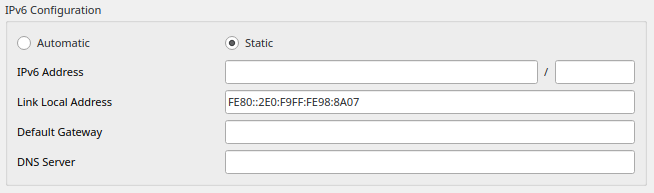
\includegraphics[height=3.75cm]{host-static-conf}
		\caption{Configuración IPv6 estática de \devname{PC0}.}
		\label{fig:host-static-conf}
	\end{figure}

	Esta dirección es una sugerencia que IPv6 nos acerca mediante una herramienta llamada \textsc{EUI-64}.  Me permite tomar la dirección MAC de 48 bits---una dirección que, al menos en teoría, ya debería ser única---y obtener un identificador único de 64 bits, el cual encaja correctamente dentro del interface ID en una dirección IPv6.

	EUI-64 funciona de la siguiente manera:  Agarro la dirección MAC de la interface y la separo a la mitad.  En el medio de ambas partes inserto la constante \ipaddress{ff:fe}, y luego uno las tres.  Finalmente, tomo el séptimo bit desde la izquierda de la dirección y lo invierto, obteniendo el identificador final.

	En la configuración de \devname{PC0}, vemos que su dirección MAC es \macaddress{00:e0:f9:98:8a:07}.  Entonces, EUI-64 la transforma de la siguiente manera:
	\[\begin{array}{rl}
		\text{\starredbullet} & \macaddress{00:e0:f9:98:8a:07} \\
		\Longrightarrow & \macaddress{00:e0:f9} + \macaddress{98:8a:07} \\
		\Longrightarrow & \macaddress{00:e0:f9} + \macaddress{ff:fe} + \macaddress{98:8a:07} \\
		\Longrightarrow & \macaddress{00000000:e0:f9} + \macaddress{ff:fe} + \macaddress{98:8a:07} \\
		\Longrightarrow & \macaddress{00000010:e0:f9} + \macaddress{ff:fe} + \macaddress{98:8a:07} \\
		\Longrightarrow & \macaddress{02:e0:f9} + \macaddress{ff:fe} + \macaddress{98:8a:07} \\
		\Longrightarrow & \macaddress{02:e0:f9:ff:fe:98:8a:07}
	\end{array}\]
	Toda dirección de enlace local comienza con el prefijo \ipaddress{fe80::/10}.  Entonces, si combinamos este prefijo con el identificador EUI-64, y de paso comprimimos la dirección, llegamos al resultado que ya teníamos:

	\[\therefore \macaddress{fe80::2e0:f9ff:fe98:8a07}\]

	\pant

	Veamos entonces cómo es la configuración automática.  En el mismo panel de la Figura \ref{fig:host-static-conf} seleccionamos \textit{Automatic}.

	Inmediatamente, \devname{PC0} confecciona un mensaje de tipo \texttt{0x85}, llamado \textit{Router Solicitation} (RS)---ilustrado en la Figura \ref{fig:icmp-rs}---y se lo envía a \devname{Switch0}.  En este mensaje, la IP de origen es la dirección de enlace local que habíamos obtenido automáticamente mediante EUI-64, y la dirección de destino es otra dirección especial, \ipaddress{ff02::2}, tambien llamada \textit{all-routers multicast}.  Habría sido valido tambien si \devname{PC0} hubiese envíado \ipaddress{::/128} como su dirección de origen---que representa una IP no asignada---pero ambas opciones funcionan.

	\begin{figure}
		\centering
		\begin{bytefield}{32}
			\bitbox{4}{Ver. 6} & \bitbox{8}{TFRC} & \bitbox{20}{Flow label} \\
			\bitbox{16}{Payload length:  12 bytes} & \bitbox{8}{Next: 0x3a} & \bitbox{8}{Hop lim.: 255} \\
			\wordbox{4}{Source IP:  \ipaddress{fe80::2e0:f9ff:fe98:8a07}} \\
			\wordbox{4}{Destination IP:  \ipaddress{ff02::2}} \\

			\\

			\bitbox{8}{Type: 133\\\scriptsize{Router Sol.}} & \bitbox{8}{Code: 0} & \bitbox{16}{Checksum: 0} \\
			\wordbox{1}[bgcolor=lightgray]{} \\
			\wordbox{1}[bgcolor=lightgray]{}
		\end{bytefield}
		\caption{Router Solicitation de \devname{PC0}.}
		\label{fig:icmp-rs}
	\end{figure}

	El mensaje viaja de \devname{PC0} a \devname{Switch0}, luego, llega hacia \devname{Router0}, quien lo acepta.  En respuesta a esto, \devname{Router0} envía un mensaje de \textit{router advertisement} tal y como habíamos discutido previamente.  Este mensaje se comporta de igual manera---su origen es \ipaddress{fe80::1} y su destino es \ipaddress{ff02::1}.  La respuesta viaja a todos los nodos---o en este caso a \devname{Switch0}, y llega de vuelta a \devname{PC0}.

	Cuando \devname{PC0} recibe la respuesta, puede intentar autoconfigurarse.  Sabe que el default gateway será \ipaddress{fe80::1}, asi que puede completar ese campo.  También recibió la porción de red de la dirección, \ipaddress{2001:db8:acad:1::/64}, y utilizando el mismo identificador que usó para rellenar su dirección de enlace local, va a intentar combinar estas dos partes para obtener una dirección GUA (\textit{Global Unique Address}).  Así, puede completar el campo con \ipaddress{2001:db8:acad:1:2e0:f9ff:fe98:8a07/64}.

	\begin{figure}
		\centering
		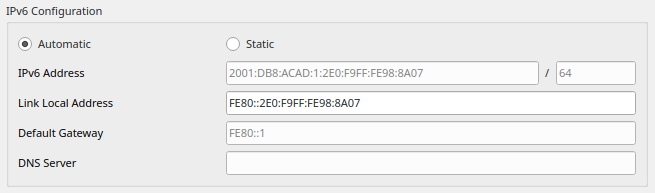
\includegraphics[height=3.75cm]{host-automatic-conf}
		\caption{Configuración IPv6 automática de \devname{PC0}.}
	\end{figure}

	Ahora, el último paso:  Dado que las direcciones de \devname{PC0} fue generada sin saber si estaba ocupada, es necesario asegurarse que ningún otro dispositivo ya las estén usando.  Para hacer esto, \devname{PC0} va a enviar un mensaje \textit{Neighbor Solicitation} (NS) para asegurarse que nadie más esté usando la IP que quiere usar---esto no es todo lo que hacen los mensajes NS y NA, eso lo veremos en el siguiente Capítulo.

	\devname{PC0} quiere saber si su IP está disponible en la red.  Para ello, va a enviar un mensaje NS con una IP de origen sin especificar (\ipaddress{::/128}) y va a poner como destino el \textit{all-solicited nodes multicast} con los últimos 24 bits de su dirección IP tentativa.  Es decir, en lugar de usar una dirección `broadcast' o usar \ipaddress{ff02::1} de nuevo, va a usar la dirección \ipaddress{ff02::1:ff98:8a07}---que significa ``todos los nodos cuya IP de enlace local termine con \ipaddress{90:9a07},'' reduciendo el tráfico.

	Si un host recibe y es el objetivo de un NS, va a responder con un mensaje de \textit{Neighbor Advertisement} (NA).  Entonces, si \devname{PC0} recibe una respuesta a su NS, sabe que la dirección IP ya está ocupada e intentará generar otra, enviando otro NS.  Si no recibe una respuesta---como será el caso en esta red---entonces puede asumir que ningún vecino ocupa su dirección, y puede finalmente apropiarse de la misma.

\renewcommand{\scenarioheight}{16\baselineskip}
\chapter{Entrega de paquetes}
	\lettrine[lraise=0.25]{¿S}{i no usamos} el protocolo ARP, cómo obtenemos las direcciones MAC?  Recordamos que, para poder transmitir mensajes, en IPv4 necesitabamos usar ARP para resolver la dirección MAC del dispositivo con la IP de destino para poder transmitir los paquetes mediante la Capa 2.  Si en IPv6 no utilizamos ARP, ¿cómo transmitimos los mensajes?

	La respuesta está en el \textit{Neighbor Discovery Protocol} (NDP), contenido dentro de la suite IPv6.  Este protocolo define algunos tipos de mensajes que permiten obtener la información de ruteo y comunicado dentro de una red.  Ya hemos estado viendo estos paquetes---vimos Router Solicitation y Router Advertisement, y tocamos un poco sobre Neighbor Solicitation y Neighbor Advertisement sin profundizar en ellos.  Estos últimos dos los vimos solo dentro del marco de SLAAC para evitar direcciones IP duplicadas, pero no mencioné que este tipo de mensajes son principalmente el mecanismo de IPv6 para determinar las direcciones de enlace de los dispositivos de la red.

	Veamos el siguiente escenario para ver cómo funciona NDP:  Tenemos dos redes, \ipaddress{2001:db8:acad:1::/64} y \ipaddress{2001:db8:acad:2::/64}.  En la primer red tenemos dos computadoras conectadas a un switch, y en la segunda una sola computadora conectada a otro switch.  \devname{Router0} es el enlace entre ambas redes, y cada host lo considera como su default gateway.
	\begin{figure}[h]
		\centering
		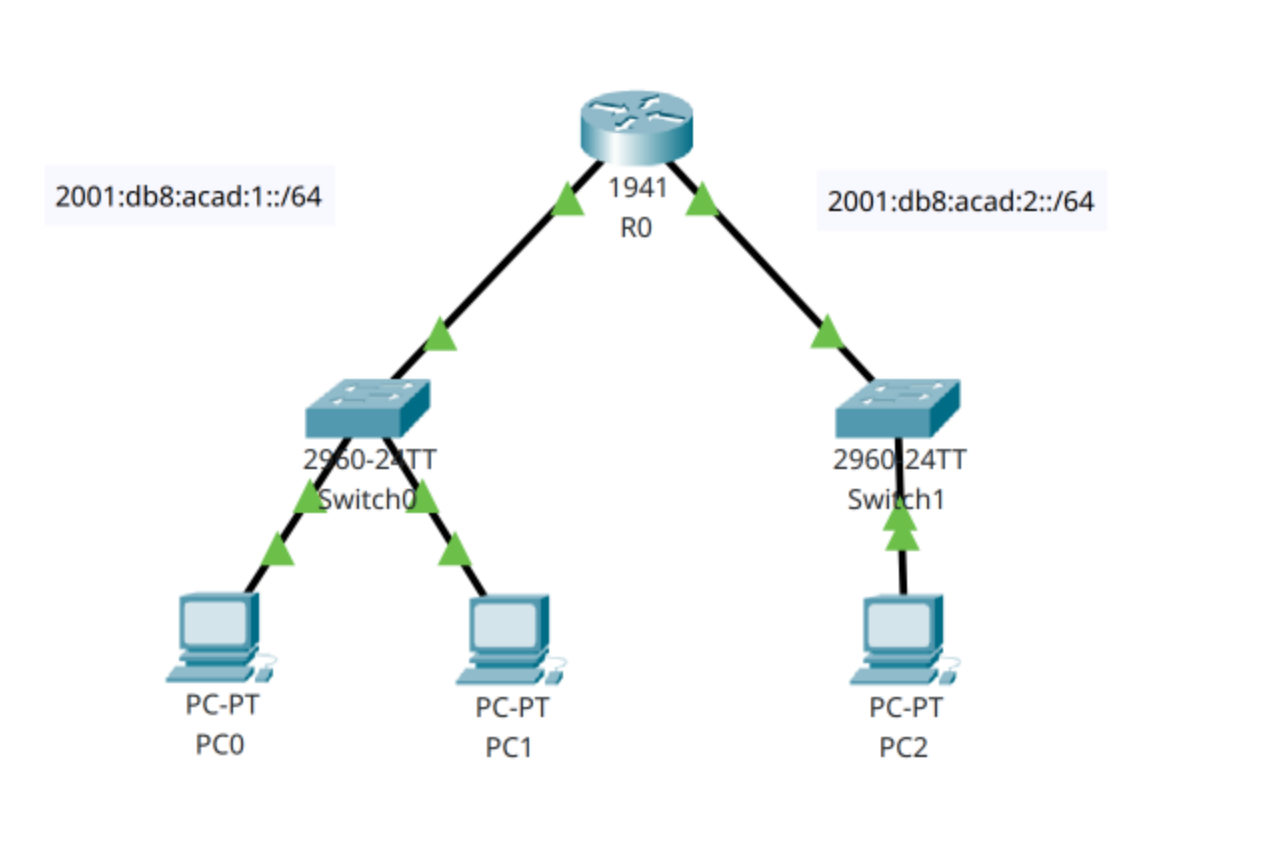
\includegraphics[height=\scenarioheight]{nd-quiet}
	\end{figure}

	Recordamos que, en IPv4, los procedimientos para la entrega local y la entrega remota eran parecidos, pero no iguales.  En IPv6 sucede lo mismo, por lo que vale la pena estudiar NDP en ambos contextos, partiendo de un estado donde todos los dispositivos saben nada acerca de sus vecinos.

	\Needspace{6\baselineskip}
	\section{Entrega local}
		\lettrine{V}{eamos primero lo} que pasa cuando \devname{PC0} le envía un ping a \devname{PC1}, siendo ambas dos computadoras dentro del mismo enlace local.  La dirección IPv6 de \devname{PC0} es \ipaddress{2001:db8:acad:1::a}, y la dirección de \devname{PC1} es \ipaddress{2001:db8:acad:1::b}, entonces ejecutamos en la consola:
		\begin{console}
			\verb|C:\> ping -n 1 2001:db8:acad:1::b|
		\end{console}

		Para realizar esta simple comunicación van ocurrir un total de trece eventos de tráfico de paquetes.  Algunos de estos paquetes son de tipo ICMPv6---porque \texttt{ping} envía este tipo de paquetes---pero los demás son de tipo NDP---porque para transmitir mediante la Capa 2 necesito averiguar las direcciones MAC.  Entremos en detalle:

		\begin{itemize}
			\item \texttt{ping} en \devname{PC0} va a crear un pedido \textit{ICMP Echo Request} (128) para buscar la respuesta de la IP de destino.  La IP de salida va a ser la IP de la interface de \devname{PC0} por la cual se va a emitir el mensaje, es decir, \ipaddress{2001:db8:acad:1::a}.  En la Capa 2, como la dirección de salto es unicast, el host va a buscar si ya conoce la dirección MAC de destino en su tabla de vecinos para poder emitir el mensaje---sin embargo, no la encuentra, y no puede enviar el paquete.

			\item En ese mismo instante, el proceso NDP de \devname{PC0} va a elaborar un mensaje de Neighbor Solicitation para la IP \ipaddress{2001:db8:acad:1::b}.  En este mensaje---visualizado en la Figura \ref{fig:icmp-ns}---la IP de origen va a ser la misma IP de \devname{PC0}, y la IP de destino va a ser el all-solicited nodes multicast con la IP de \devname{PC1}, es decir, \ipaddress{ff02::1:ff00:b}.  Notamos que esto es diferente al mensaje ICMP Echo que teníamos previamente, donde la dirección de destino era un unicast hacia \devname{PC1}.  Este mensaje, para poder ser transmitido mediante la Capa 2, necesita una dirección MAC, por lo que \devname{PC0} utiliza una dirección MAC multicast de \macaddress{33:33:ff:00:00:0b}.  La misma se forma agregando ``\macaddress{33:33}'' antes de los últimos 32 bits de la dirección IPv6 a todos los nodos solicitados.  Este mensaje sale hacia \devname{Switch0}.

			\begin{figure}
				\centering
				\begin{bytefield}{32}
					\bitbox{4}{Ver. 6} & \bitbox{8}{TRFC} & \bitbox{20}{Flow label} \\
					\bitbox{16}{Payload length:  28 bytes} & \bitbox{8}{Next: 0x3a} & \bitbox{8}{Hop lim.: 255} \\
					\wordbox{4}{Source IP:  \ipaddress{2001:db8:acad:1::a}} \\
					\wordbox{4}{Destination IP:  \ipaddress{ff02::1:ff00:b}} \\

					\\

					\bitbox{8}{Type: 135\\\scriptsize{Nbor. Sol.}} & \bitbox{8}{Code: 0} & \bitbox{16}{Checksum: 0} \\
					\bitbox{1}{R} & \bitbox{1}{S} & \bitbox{1}{O} & \bitbox{29}[bgcolor=lightgray]{} \\
					\wordbox{2}{Target address:  \ipaddress{2001:db8:acad:1::b}} \\

					\\

					\bitbox{8}{Type: 1\\\scriptsize{Link layer}} & \bitbox{8}{Length: 1} & \bitbox[lrt]{16}{} \\
					\wordbox[lrb]{1}{MAC Address:  \macaddress{00:90:2b:89:2d:86}}
				\end{bytefield}
				\caption{Neighbor Solicitation de \devname{PC0}.}
				\label{fig:icmp-ns}
			\end{figure}

			\item \devname{Switch0} recibe el paquete en \devname{FastEthernet0/1}.  Como no conocía la dirección MAC del dispositivo conectado a ese puerto, la anota en su tabla de direccionamiento.  Este switch opera en la Capa 2, por lo que no accede a la información de las capas superiores.  Como el contenido de la Capa 2 es una dirección multicast, la deja intacta y la difunde a todos sus puertos de la VLAN, salvo el puerto por donde entró el mensaje---En términos prácticos, el mensaje es reenviado a \devname{Router0} y a \devname{PC1}.

			\item \devname{PC1} recibe el mensaje de \devname{Switch0}, lee la información de la Capa 2, y verifica que está incluido dentro del multicast de destino.  Desencapsula el mensaje Capa 3, y encuentra una solicitud de vecino a su IP.  Con los datos que ya recibió a partir de este mensaje, puede actualizar su tabla de vecinos y hacer corresponder la IP de \devname{PC0} con la MAC de este paquete.  Luego, va a formular una respuesta de tipo Neighbor Advertisement---en la misma, la dirección IP de origen será la IP de \devname{PC1}, \ipaddress{2001:db8:acad:1::b}, y lo mismo con la MAC de origen, que vale \macaddress{00:90:0c:5b:e7:dc}.  Como ya conoce la IP y la MAC de \devname{PC0} puede directamente escribirlas en la respuesta como \ipaddress{2001:db8:acad:1::a} y \macaddress{00:90:2b:98:2d:86} respectivamente.  La respuesta viaja hacia \devname{Switch0}.

			\begin{figure}
				\centering
				\begin{bytefield}{32}
					\bitbox{4}{Ver. 6} & \bitbox{8}{TRFC} & \bitbox{20}{Flow label} \\
					\bitbox{16}{Payload length:  28 bytes} & \bitbox{8}{Next: 0x3a} & \bitbox{8}{Hop lim.: 255} \\
					\wordbox{4}{Source IP:  \ipaddress{2001:db8:acad:1::b}} \\
					\wordbox{4}{Destination IP:  \ipaddress{2001:db8:acad:1::a}} \\

					\\

					\bitbox{8}{Type: 136\\\scriptsize{Nbor. Advert.}} & \bitbox{8}{Code: 0} & \bitbox{16}{Checksum: 0} \\
					\bitbox{1}{R} & \bitbox{1}{S} & \bitbox{1}{O} & \bitbox{29}[bgcolor=lightgray]{} \\
					\wordbox{2}{Target address:  \ipaddress{2001:db8:acad:1::a}} \\

					\\

					\bitbox{8}{Type: 1\\\scriptsize{Link layer}} & \bitbox{8}{Length: 1} & \bitbox[lrt]{16}{} \\
					\wordbox[lrb]{1}{MAC Address:  \macaddress{00:90:0c:5b:e7:dc}}
				\end{bytefield}
				\caption{Neighbor Advertisement de \devname{PC1}.}
			\end{figure}

			\item \devname{Router0} recibe el mensaje de \devname{Switch0}, lo desencapsula, y ve que la IP que se está solicitando no es la IP suya.  Como \devname{Router0} únicamente conecta a esta red mediante \devname{Switch0}, no tiene ningún otro lado al cual redirigir el mensaje.  Por lo tanto, lo descarta, y no envía ningún paquete.

			\item \devname{Switch0} recibe la respuesta de \devname{PC1}.  Como no conocía la dirección MAC del dispositivo conectado a esa interface, también la agrega a su tabla de direcciones MAC.  Analiza la MAC de destino del mensaje, y como ya la conoce, envía la respuesta directamente hacia \devname{PC0}.

			\item \devname{PC0} recibe el Neighbor Advertisement de \devname{PC1}, y agrega en su tabla de vecinos que la dirección IP \ipaddress{2001:adb8:acad:1::b} corresponde a la MAC \macaddress{00:90:0c:5b:e7:dc}.  Efectivamente, ya tiene toda la información que necesita para comunicarse con \devname{PC1}.

			\item Ahora, \devname{PC0} retoma el mensaje de tipo ICMP Echo que había querido enviar según la orden del comando \texttt{ping}.  Completa la dirección MAC de destino que le faltaba, como se puede ver en la Figura \ref{fig:icmp-echo-request}, y envía el mensaje hacia \devname{Switch0}.

			\begin{figure}
				\centering
				\begin{bytefield}{32}
					\bitbox{4}{Ver. 6} & \bitbox{8}{TRFC} & \bitbox{20}{Flow label} \\
					\bitbox{16}{Payload length:  108 bytes} & \bitbox{8}{Next: 0x3a} & \bitbox{8}{Hop lim.: 255} \\
					\wordbox{4}{Source IP:  \ipaddress{2001:db8:acad:1::a}} \\
					\wordbox{4}{Destination IP:  \ipaddress{2001:db8:acad:1::b}} \\

					\\

					\bitbox{8}{Type: 128\\\scriptsize{Echo request}} & \bitbox{8}{Code: 0} & \bitbox{16}{Checksum: 0} \\
					\bitbox{16}{Identifier: 3} & \bitbox{16}{Sequence number: 2} \\

					\\

					\wordbox{2}{Data (100 bytes, achicado)}
				\end{bytefield}
				\caption{Mensaje ICMP Echo Request que \devname{PC0} le enviará a \devname{PC1}.}
				\label{fig:icmp-echo-request}
			\end{figure}

			\item \devname{Switch0} le transmite el mensaje a \devname{PC1}.

			\item \devname{PC1} recibe el pedido y le envía una respuesta otra vez a la IP de origen mediante \devname{Switch0}.  Esta respuesta es de tipo \textit{ICMP Echo Reply} (129), como se puede ver en la Figura \ref{fig:icmp-echo-reply}.

			\begin{figure}
				\centering
				\begin{bytefield}{32}
					\bitbox{4}{Ver. 6} & \bitbox{8}{TRFC} & \bitbox{20}{Flow label} \\
					\bitbox{16}{Payload length:  108 bytes} & \bitbox{8}{Next: 0x3a} & \bitbox{8}{Hop lim.: 255} \\
					\wordbox{4}{Source IP:  \ipaddress{2001:db8:acad:1::b}} \\
					\wordbox{4}{Destination IP:  \ipaddress{2001:db8:acad:1::a}} \\

					\\

					\bitbox{8}{Type: 129\\\scriptsize{Echo reply}} & \bitbox{8}{Code: 0} & \bitbox{16}{Checksum: 0} \\
					\bitbox{16}{Identifier: 3} & \bitbox{16}{Sequence number: 2} \\

					\\

					\wordbox{2}{Data (100 bytes, achicado)}
				\end{bytefield}
				\caption{Mensaje Echo Reply de \devname{PC1} a \devname{PC0}.}
				\label{fig:icmp-echo-reply}
			\end{figure}

			\item \devname{Switch0} le transmite el mensaje a \devname{PC0}.

			\item \devname{PC0} recibe la respuesta a su solicitud \texttt{ping}.  Muestra en la pantalla que la conexión se logró realizar y el tiempo real que demoró en comunicarse.
		\end{itemize}

		\pant

		Este método para resolver las direcciones MAC a partir de IP toma ventaja de la emisión de mesanjes multicast en lugar de inundar toda la red con broadcasts.  Además, como ya debería ser familiar para nosotros, sabemos que \devname{PC0} y \devname{PC1} han almacenado la dirección MAC de la otra máquina en una tabla local, y van a mantener esa información por cierto tiempo.  Entonces, la próxima vez que ejecutemos el mismo comando \texttt{ping}, vamos a ver que los mensajes NDP no son emitidos, ya que \devname{PC0} tiene una asociación de la IP de \devname{PC1} a su MAC.  El mensaje viaja de \devname{PC0} a \devname{Switch0} a \devname{PC1}, y la respuesta de \devname{PC1} a \devname{Switch0} a \devname{PC0} de vuelta.

		Por supuesto, la información en la tabla de vecindad no es inmutable.  Si \devname{PC0} no hubiese recibido una respuesta de \devname{PC1}---por un corte en la red, porque el host estaba apagado, etc---\devname{PC0} hubiese borrado la entrada con la IP de \devname{PC1} de su tabla de vecindad e intentaría buscar la dirección MAC de la IP de destino otra vez usando el mismo protocolo NDP.  También es posible que se borren las entradas de la tabla de vecindad en un host luego de que haya transcurrido bastante tiempo---porque ya podría ser razonable que el estado del resto de la red haya cambiado lo suficiente como para dejar obsoleta la información que el host tenía previamente.

		De esta forma, no se envían mensajes NDP muy redundantes, lo que acelera un poco la comunicación inicial y reduce el tráfico general en la red.

	\section{Entrega remota}
		\lettrine{N}{o resulta el} caso que podemos usar exactamente los mismos pasos para la entrega local si queremos enviar un paquete a un dispositivo fuera de nuestra red.  Si, el procedimiento es medio parecido---y no es tan alien a como funcionaba en IPv4---pero es importante entender cómo y por qué funciona como funciona el mecanismo de entrega remota de paquetes en IPv6.

		Vamos a reiniciar la simulación, usando el mismo escenario que antes en un punto donde ninguno de los dispositivos sabe algo de sus vecinos, y vamos a intentar hacer un ping a \devname{PC2} desde \devname{PC0} mediante el siguiente comando:
		\begin{console}
			\verb|C:\> ping -n 1 2001:db8:acad:2::a|
		\end{console}

		\begin{itemize}
			\item Primero, \texttt{ping} va a crear un ICMP Echo Request para enviarlo a la dirección de destino.  Luego, va a comparar la porción de red de la dirección IP de \devname{PC0} contra la porción de red de la dirección de destino.  Nosotros no le especificamos la porción de red de esta dirección, pero \texttt{ping} simplemente le aplica misma máscara que la de la porción de red de la IP de \devname{PC0}.  Lo que va a observar es que ambas IP están en redes diferentes, por lo tanto, se debe usar el mecanismo de entrega remota, y enviar el mensaje al default gateway.

			\item Entonces, \devname{PC0} va a preparar un mensaje NDP de Neighbor Solicitation con origen en su dirección de enlace local---\ipaddress{fe80::290:2bff:fe89:2d86}---cuyo objetivo es la IP del default gateway y su dirección de destino es un multicast dirigido a esa IP (\ipaddress{ff02::1:ff00:1}).  Esta parte del mecanismo es muy similar a la de entrega local---simplemente estamos resolviendo la MAC del default gateway.

			\item Resumiendo entonces la parte del mecanismo que recién acabamos de ver, \devname{PC0} consigue la dirección MAC de \devname{Router0}---\macaddress{00:0d:bd:9d:bc:01}---y termina de preparar el mensaje ICMP Echo; completando la dirección MAC de destino con la de \devname{Router0}, y completando la MAC de origen con la suya, \macaddress{00:90:2b:89:2d:86}.

			\item El mensaje viaja de \devname{PC0} a \devname{Switch0}, luego, llega a \devname{Router0}.  Este router conecta la red \ipaddress{2001:db8:acad:1::/64} con la red \ipaddress{2001:db8:acad:2::/64}, que es a donde debe enviarse el mensaje.  \devname{Router0} podrá enviar el mensaje, pero todavía no conoce la dirección MAC.  Por lo tanto, va a generar un Neighbor Solicitation nuevo para resolver la dirección MAC de \devname{PC2}.  Este mecanismo, de nuevo, es el mismo que ya habíamos visto, simplemente que esta vez es el router quien comienza la solicitud.

			\item \devname{Router0} consigue la dirección MAC correspondiente a la IP de destino del paquete, \macaddress{00:0a:41:e4:42:d4}.  \devname{Router0} le envía el mensaje a \devname{Switch1}, quien se lo hace llegar finalmente a \devname{PC2}.

			\item \devname{PC2} recibe un ICMP Echo Request proveniente de una IP que no conoce.  Como corresponde según el protocolo, comenzará a preparar un mensaje tipo ICMP Echo Reply para enviar a la IP de origen, pero no lo podrá enviar porque hasta que encuentre la dirección MAC del dispositivo al cual debe enviarlo.  Primero---y de mismo modo que hizo \devname{PC0}---compara las porciones de red de ambas direcciones IP y concluye que están en redes distintas, por lo que debe enviar el mensaje a la MAC del default gateway.  Sin embargo, no conoce esta dirección, por lo que comienza otro proceso NDP para conseguirla.

			\item Entonces \devname{PC2} envía un ICMP Echo Reply con dirección MAC de destino en \devname{Router0}.  El mensaje pasa por \devname{Switch1}, y luego llega al router, quien mediante NDP resuelve la MAC de \devname{PC0}.  Finalmente, el router le dirige la respuesta del \devname{PC2} a \devname{PC0}, quien muestra los resultados en la pantalla.
		\end{itemize}

		\pant

		Aquí, ahora, sucede lo mismo que ocurrió en el caso de entrega local---dado que se resolvieron hace poco las direcciones MAC de los dispositivos que me importan, si reseteo la simulación y vuelvo a ejecutar el mismo comando \texttt{ping}, me puedo omitir los pasos de resolución de MACs.  No solo eso, sino que, como la red está usando switches, en esta segunda vuelta los mensajes se enviarán directamente a los dispositivos que corresponde---no hace falta hacer ningun broadcast o multicast.

		Cuando vuelvo a ejecutar \texttt{ping}, únicamente envio mensajes ICMPv6---y este ahorro de mensajes NDP se puede ver en que la respuesta del ping demora menos tiempo en llegar.  \devname{PC0} envía el mensaje directamente a su default gateway, \devname{Router0}, y con \devname{PC2} lo mismo.  Ambos dispositivos saben las direcciones que necesitan para poder comunicarse con un dispositivo que está en una red remota.

		\rest

		También podemos ir a \devname{Router0} y consultarle qué aprendió sobre sus vecinos:
		\begin{console}
			\begin{verbatim}R0# show ipv6 neighbors
IPv6 Address                           Age Link-layer Addr State Interface
2001:DB8:ACAD:1::A                       0 0090.2B89.2D86  REACH Gig0/0
2001:DB8:ACAD:2::A                       0 000A.41E4.42D4  REACH Gig0/1
FE80::20A:41FF:FEE4:42D4                 0 000A.41E4.42D4  REACH Gig0/1
FE80::290:2BFF:FE89:2D86                 0 0090.2B89.2D86  REACH Gig0/0\end{verbatim}
		\end{console}

		Hay cuatro direcciones, y como están ordenadas de menor a mayor es menos inmediato de ver que estas direcciones son las dos direcciones IP de los dos dispositivos que se comunicaron mediante \texttt{ping}:  En la interface \devname{GigabitEthernet0/0} estaba \devname{PC0}, cuya dirección local era \ipaddress{fe80::290:2bff:fe89:2d86}, que \devname{Router0} aprendió porque fue la dirección que \devname{PC0} uso para el proceso NDP, y también conoce su dirección GUA, \ipaddress{2001:db8:acad:1::a}, ya que es la que usó para el ping.  Puede asociar que estas dos direcciones corresponden al mismo dispositivo, porque en la tabla muestra que debe rutear ambas direcciones a la misma dirección MAC, \macaddress{00:90:2b:89:2d:86}.

		Análogamente, pasa lo mismo con las entradas de las direcciones de \devname{PC2}.

		Podemos tomar nota también de la cuarta columna, \texttt{STATE}.  Actualmente nos indica que todos las entras han respondido a un intento de comunicación reciente---lo que tiene sentido, porque recién acabamos de comunicarnos con \texttt{ping}---pero también podría indicar, por ejemplo, que no se ha recibido ninguna comunicación con ese dispositivo en mucho tiempo, o que NDP falló en resolver esas direcciones MAC y se consideran inalcanzables, etc.  Es gracias a esta información que podemos ahorrarnos el tiempo extra de volver a realizar un proceso NDP.

		Lo que no podemos ver es ninguna entrada que se relacione con \devname{PC1}---que tiene sentido, desde que reseteamos la simulación y borramos todas las tablas de vecindad, \devname{PC1} no envió ningún paquete, solamente rechazó algnos paquetes que \devname{Switch0} le brodcasteó.  Sin embargo, podríamos hacer que \devname{PC1} aparezca en la tabla enviandole un ping:
		\begin{console}
			\begin{verbatim}R0# ping 2001:db8:acad:1::b

Type escape sequence to abort.
Sending 5, 100-byte ICMP Echos to 2001:db8:acad:1::b:
!!!!!
Success rate is 100 percent (5/5), round-trip min/avg/max = 0/0/4 ms

R0#show ipv6 neighbors
IPv6 Address                           Age Link-layer Addr State Interface
2001:DB8:ACAD:1::A                       0 0090.2B89.2D86  REACH Gig0/0
2001:DB8:ACAD:1::B                       0 0090.0C5B.E7DC  REACH Gig0/0
2001:DB8:ACAD:2::A                       0 000A.41E4.42D4  REACH Gig0/1
FE80::20A:41FF:FEE4:42D4                 0 000A.41E4.42D4  REACH Gig0/1
FE80::290:2BFF:FE89:2D86                 0 0090.2B89.2D86  REACH Gig0/0\end{verbatim}
		\end{console}

		Aquí, \devname{Router0} vio que tiene una interface que se conecta a la red \ipaddress{2001:db8:acad:1::/64}, donde está contenida la dirección del dispositivo al que quería llegar.  Por lo tanto, ejecutó el mecanismo de entrega local---esto es porque solo me importa el prefijo de red para saber qué mecanismo uso, no me importa saber si es una dirección GUA o LLA.

		Algo para notar es que \textit{podría} haber usado una LLA, pero si ese fuera el caso la mejor práctica hubiese sido especificar también la interface---una LLA sólo es válida dentro de un dominio de broadcast, por lo tanto, en dos dominios de broadcast distintos podrían aparecer dos direcciones LLA que coincidan.  Si este hubiese sido el caso en \devname{Router0}, no podría haber hecho el ping, ya que queda ambiguo a qué dispositivo me estaba refiriendo---si era \ipaddress{fe80::x\%Gig0/0} o \ipaddress{fe80::x\%Gig0/1}.

\chapter{Conclusiones}
	\lettrine{E}{l protocolo IPv6} es la versión más reciente del protocolo IP, diseñado para resolver el problema del agotamiento de las direcciones IPv4.  Hoy vimos cómo funcionan los mecanismos de comunicación para los dispositivos de red bajo este protocolo, observamos las ventajas inmediatamente aparentes, como el uso de SLAAC para la autoconfiguración correcta de dispositivos, y el reemplazo de broadcasts por multicasts dirgidos, para reducir el tráfico innecesario en la red.

	Se puede ver claramente reflejado la filosofía bajo la cual este protocolo fue diseñado, y el rol que sus desarolladores querían que cumpla---ser escalable a muy largo plazo.  Esto es definitivamente una ventaja, porque no se espera que se llegue algún día a vivir un agotamiento de direcciones IPv6 antes que el protocolo sea reemplazado por uno del futuro, y porque las direcciones tienen tantos bits que puedo tener muchas subredes y jerarquías sin tener que sacrificar la cantidad de dispositivos que pueden conectarse a ellas.  El uso de 128 bits para las direcciones IP es definitivamente una ventaja.  Probablemente una desventaja---a simple vista no parece tanto, pero con tanto tráfico de paquetes termina sumando---es que justamente estamos usando cuatro veces más bits para las direcciones IP comparado a lo que usabamos en IPv4.  Esto significa que los encabezados de los paquetes son más largos, las computadoras deben tomar más trabajo para almacenar estas direcciones, y si es un humano en la terminal escribiendo una dirección a mano tiene muchas más oportunidades para cometer un error.  Con los sistemas modernos el costo computacional para un host de manejar más bits para la IP probablemente no valga tanto, pero puede generar un gran desafío para el hardware más antiguo.

	Para la autoconfiguración, se usan principalmente los mensajes de Router Solicitation y Router Advertisement.  Para el descubrimiento  de direcciones de la Capa 2 se usan los Neighbor Solicitation y Neighbor Advertisement.  Los RS y RA se usan para la confoiguración de la parte de red, y---con ayuda de los mensajes NS---luego detectar si una dirección está o no ocupada.  El uso principal de los mensajes NS y NA es para resolver direcciones MAC, pero como hemos visto esto tambien se puede usar para el detectado automatico de direcciones duplicadas.  Podemos decir que lo que tienen en común ambos tipos de mensajes es que buscan resolver información de direccionamiento sobre distintas capas---Los RS y RA sirven para resolver las direcciones IP, y los NS y NA sirven para resolver las direcciones MAC.

	Un dispositivo requiere realizar el proceso de deteccion de vecinos siempre y cuando quiera transmitir un mensaje IPv6 mediante la red y no conozca la MAC del dispositivo local al que deba enviarlo.  Por lo general, una vez que realiza este proceso puede almacenar las respuestas de la detección por bastante tiempo ya que es probable que no cambien si no hay una pausa prolongada en la comunicación.  También, de nuevo, mencionamos que el proceso de detección de vecinos también se usa para que no hayan direcciones IP duplicadas.

	Los routers ayudan a minimizar el tráfico ND en la red manteniendo la información de la tabla de vecindad generalmente actualizada.  Los routers no redirigen mensajes NDP innecesarios y periódicamente suelen enviar mensajes RA para asegurarles a los hosts que tienen un gateway para la conexión a dispositivos de forma remota.  El impacto de NDP en los hosts también está minimizado, debido a que ellos tambien mantienen una tabla de vecindad, y tanto los hosts como los routers no envían mensajes broadcast para NDP, sino que envían mulitcasts dirigidos a los dispositivos cuyas direcciones podrían ser el objetivo.

\end{document}
